\chapter{مبادئ الكتابة بلغة الليتك}
\section{ماهي لغة الليتك}
الليتك
\textenglish{\LaTeX}
 لغة مجانية مفتوحة المصدر تستخدم لتنسيق الكتابة بكافة انواعها سواء كانت كتاب مقالة رسالة تقرير او شرائح عرض بشكل احترافي باستخدام قوالب جاهزة تكفي المستخدم عناء الدخول في مشاكل التنسيق. تهدف الى جعل المستخدم يهتم بالمحتوى دون الاهتمام بطريقة تنسيقه. كتبت الليتك  بواسطة ليزلي لمبارت  Leslie Lamport عام 1985  بهدف تبسيط منسق النصوص TeX المكتوب بواسطة استاذ الرياضيات الالماني دونلد نوث  Donald Knuth الذي كان يسعى لايجاد طريقة سهلة لكتابة الكتب العلمية وكتب الرياضيات على وجه الخصوص. وتعتبر لغة الليتك بشكلها الحالي مناسبة لكتابة الوثائق العلمية  والتقنية في كافة المجالات  وليست حكرا على علم الرياضيات فقط. فهي تستطيع اظهار المعادلات الرياضية والكيميائية وغيرها من الرموز على حد سواء بشكل احترافي تعجز عنه كثير من محررات النصوص التجارية. ظلّ استعمال الليتك ممكنا فقط لكتابة المقالات والكتب باللّغات التي تُكتب من اليسار إلى اليمين.  وظلّ  الليتك أعجمياً لايفهم العربيّة، إلى أن جاء كلاوس لاقلي Klaus Lagally من جامعة شتوتغارت الألمانيّة حيث زوّد الليتك بمكتبة دعاها ArabTeX، لكن هذه المكتبة لم تشمل كلّ إمكانيّات الليتك والتّعامل معها لم يزل صعبا ومعقّدا. عندما
أُصدرت نسخة جديدة من لاتيك تدعى كزيلاتك XeLaTeX تفهم النّصوص المرمّزة بنظام UTF8، ويمكنها أن تنسّق النّص من اليمين إلى اليسار ومتأقلمة مع كلّ المكتبات المخصّصة بالليتك LaTeX.بما ان التعامل مع هذه النسخة من اللتيك باللّغة العربيّة يستوجب إضافة مكتبة خاصّة بذلك قاما د. مصطفى العليوي من المعهد العالي للعلوم التطبيقية والتكنولوجيا بهذه المهمة وأضاف مكتبة سمّاها XeArabic، تبسّط استعمال XeLaTeX باللغة العربية وتختصره بشكل كبير، وذلك من أجل كتابة المقالات العلميّة والكتب والمحاضرات العربية بواسطة XeLaTeX فلاظهار المحتوى في الشكل الموضح ادناه \\
\begin{mybox}
\begin{figure}[H]
  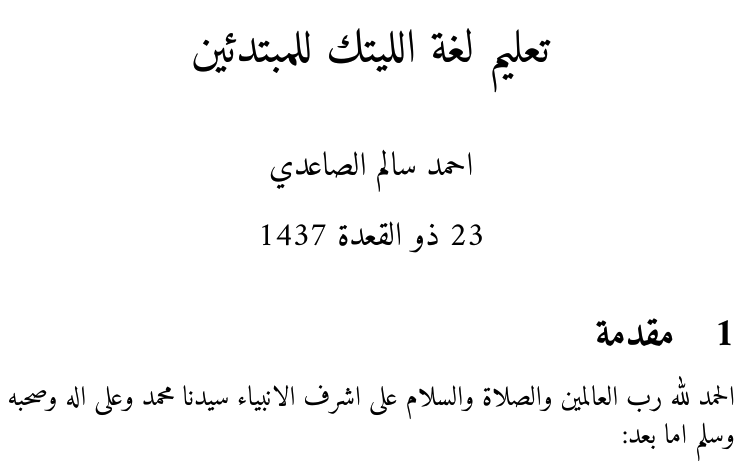
\includegraphics[width=\linewidth]{figures/example1.png}
  \caption{جزء من مقال مكتوب بالليتك \LaTeX}
  \label{fig:startpython}
\end{figure}
\end{mybox}
يتحتاج المستخدم فقظ لكتابة الكود التالي:
\begin{english}
\begin{mybox}
\textbackslash documentclass\{article\}\\
\textbackslash begin\{document\}\\
\textbackslash title\{\textarabic{تعليم لغة الليتك للمبتدئين}\}\\
\textbackslash author\{\textarabic{احمد سالم الصاعدي}\}\\
\textbackslash date\{\textbackslash today\}\\
\textbackslash section\{\textarabic{مقدمة}\}\\
\textarabic{
الحمد لله رب العالمين والصلاة والسلام على اشرف الانبياء سيدنا محمد وعلى اله وصحبه وسلم اما بعد:
}\\
\textbackslash end\{document\}
\end{mybox}
\end{english}
لاحظ ان الكود لا تحتوى على اي تنسيق ولكن تحتوي مفردات تخبر مفسر الليتك بما يجب فعله ليظهر المحتوى بما بتطلبه المستخدم
\section{لماذا نحتاج الى استخدام لغة الليتك}

ان شيوع استخدام ميكروسوفت ورد قد يدفع القارئ الى التساءل عن الاسباب التى تدعونا الى استخدام الليتك في ظل وجود برنامج تنسيق النصوص من ميكروسوفت ورد. لكي نجيب على هذا التساءل للنظر الى الشكل س ادناه. \\ 
\begin{mybox}
	\begin{figure}[H]
		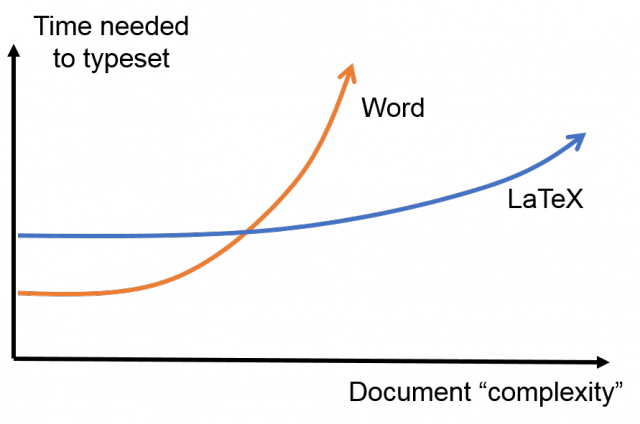
\includegraphics[width=\linewidth]{figures/mswvslatex.png}
		\caption{مقارنة بين استخدام محرر النصوص من ميكروسوفت والليتك \LaTeX}
		\label{fig:startpython}
	\end{figure}
\end{mybox}

ان استخدام ميكروسوفت ورد قد يكون اكثر سهله عند كتابة عدد قليل من الصفحات لكن عند التعامل مع عدد كبير من الصفحات فان الجهد المبذول يتضاعف بشكل كبير فتصبح عملية التنسيق مضنية ومرهقة. لكن عن استخدام لغة الليتك فان عملية الكتابة حتى ولو كان المراد كتابته يتطلب عدد كبير من الصفحات فان المجهود المبذول لعملية التنسيق يضل اقل بكثير مما هو مطلوب عند استخدام ميكروسوفت ورد. بالاضافة الى ان هناك اسباب اخرى تجعلنا نفضل لغة الليتك على منسقات النصوص الى على شاكلة ميكروسوفت ورد والتىي منها على سبيل الذكر لا الحصر :\\
\begin{itemize}
\item{حجم الملفات يكون صغير عند استخدام الليتك}
\item{الليتك مجاني مفتوح المصدر ويمكن استخدامه على جميع انظمة التشغيل المتوفرة}
\item{يمكن عمل القوالب بكل سهوله}
\end{itemize}

\section{ماهي الادوات اللتى نحتاجها لستخدام لكتابة بلغة الليتك}

للكتابة بلغة الليتك نحتاج الى مفسر للغة الليتك ونحتاج برنامج لكتابة النصوص مثل نوت باد في ميكروسوفت وندوز او تكست اديت في ماك. والافضل هو استخدام محرر خاص بلغة الليتك مثل تكس ميكر او تكس ستوديو. بالنسبة لمفسر لغة الليتك هناك اصدارة خاصة بالوندوز وهي ميك تك
هناك ايضا مايسمى بالكتابة بلغة ليتك من خلال شبكة الانترنيت حيث توجود مواقع من اشهرها شير ليتك ورايت ليتك تمكن من الكتابة مباشرة بلغة الليتك بعد التسجيل المجاني في هذه المواقع.
\section{كتابة اول مقالة بلغة الليتك}
هناك جزئين رئيسيين في لغة الليتك يجب توفرهما في الوثيقة المراد كتابتها من اجل ان تتم عملية تنسيقها. 
\\
الجزء الاول: نوع الوثيقة المراد تنسيقها ويشار اليها بالتركيب اللغوي التالي:
\\
\begin{english}
\begin{mybox}
\textbackslash documentclass\{\}
\end{mybox}
\end{english}
هذا التركيب اللغوي يحدد نوع الوثيقة المراد تنسيقها والمكتبة الرئيسية للغة الليتك تحتوي على عدة انواع من الوثائق والتي من بينها:
\begin{enumerate}
\item{article}
\item{book}
\item{letter}
\item{slide}
\item{report}
\end{enumerate}
فعندما نريد تنسيق مقالة مثلا فننا نستفتح الوثيقة بالامر التالي:
\begin{english}
\begin{mybox}
\textbackslash documentclass\{article\}
\end{mybox}
\end{english}
وعندما نريد تغيير نوع الوثيقة فاننا فقط نغير الاسم الموجود بين القوسين المتعرجين.
\\
الجزء الثاني: تحديد بداية ونهاية الوثيقة كما في المثال التالي:
\begin{english}
\begin{mybox}
\textbackslash begin\{document\}
\\
\\
\textarabic{
هنا يكتب محتوى الوثيقة
}
\\
\\
\textbackslash end\{document\}
\end{mybox}
\end{english}
والوثيقة التي تتكون من هذين الجزئين يعتبر ابسط تركيب لغوي يمكن استخدامه وبدون هذين الجزئين لايمكن تنسيق الوثيقة وسف يعطي المالج خطأ للمستخدم عند اجراء علمية المعالجة.
بين هذين الجزئين هناك جزء اختياري لكنه مهم وهو ما يسمى بجزء استخدام المكتبات وتعريف الاومر الجديدة كما هو موضح في الشكل التالي:
\begin{english}
\begin{mybox}
\textbackslash documentclass\{article\}
\\preamble
\\
\textarabic{
جزء ادراج المكتبات وتعريف الاومر الجديدة
}
\\
\textbackslash begin\{document\}
\\
\\
\textarabic{
محتوى الوثيقة يكتب هنا
}
\\
\\
\textbackslash end\{document\}
\end{mybox}
\end{english}
سوف نتطرق الى كيقية ادارج المكتبات وتعريف الاوامر في جزء لاحق من هذا الكتاب ولكن بعد ان نفصل اساسيات التركيب اللغوي في لغة الليتك:
\begin{enumerate}
\item{اسمتخدام \textbackslash في بداية كل تركيب لغوي}
كما لاحظنا في التراكيب اللغوية السابقة فان جميع اوامر لغة الليتك تستفتح بعلامة القسمة المعكوسة لتخبر المعالج بوجود يجب معالجته. فمثلا التركيب اللغوي السابق 
\begin{mybox}

\end{mybox}
يخبر المعالج بنوع الوثيقة المراد تنسيقها وهذا النوع يوضع بين قوسين كمعلومات مدخلة من المستخدم للمعالج. فالمعلومات المدخلة من المستخدم للمعالج اما ان تكون مدخلات رئيسية لابد من تزويد المعالج بها فتكتب بين قوسين متعرجين او تكون مدخلات اختيارية يمكن تنسيق الوثيقة بدونها فتوضع بين قوسين مربعين كما في المثال التالي:
\begin{mybox}

\end{mybox}
فادخال نوع الوثيقة يعتبر من المدخلات الاساسية التي تجتاجها المعالج لتنسيق الوثيقة لذلك نكتبها بين القوسين المتعرجين اما حجم خط الوثيقة فانه اختياري لذلك نضعه بين قوسين مربعين.
\item{الاحرف الكبيرة لا تشابة الاحرف الصغيرة}
لغة الليتك تهتم بما اذا كانت التراكيب اللغوية مكتوبة بالاحرف الكبيرة ام الصغيرة. فعند كتابة التركيب اللغوي لنوع الوثيقة بالاحرف الكبيرة مثلا فان المعالج يظهر للمستخدم وحود خطأ في التركيب اللغوي يجب تعديلة قبل ان يتم تنسيق الوثيقة. كما في المثال التالي:

\item{الرمور المحجوزة لاوامر لغة الليتك}
هناك رموز محجوزة لاوامر لغة الليتك لا يمكن استخدامها كمحتوى في الوثيقة الا اذا ادرجنا قبل هذا الرمز رمز القسمة المعكوسة لان هذه العلامة او الرمز تخبر المعالج ان يتجاهل هذا الرمز يدرجه كمحتوى في الوثيقة ومن الامثلة على الرموز المحجوزة للغة الليتك مايلي:
\\ هنا تكتب الرموز

فعند كتابة الرمز س مثلا فان المعالج يتعامل معه كامر تنسيق ام اذا تم اداراج القسمة المعكوسة قبله فان المعالج يدرج الرمز كجزء من المحتوى كما في المثال التالي:
\begin{mybox}

\end{mybox}
\item{ادراج الملاحظات على الوثيقة}
لادارج ملاحظات تذكر المستخدم بما ينوى عمله او كتابته باستخدام الرمز "٪" فجميع محتويات السطر التي يسبقبها علامة النسبة المئوية يتجاهلها المعالج يعتبرها ملاحظات للتذكير المستخدم ولا تظهر في محتوى الوثيقة كما في المثال التالي:
\begin{mybox}

\end{mybox}
\item{الفراعات في الوثيقة}
يتجاهل المعالج الفراغات داخل السطر الواحد ويعتبر بفراغ واحد فقط كما في المثال التالي:
\begin{mybox}

\end{mybox}
\item{الاسطر الفارغة في الوثيقة}
ادراج اسطر فارغة في الوثيقة يتجاهله المعالج ولا يظهر في محتوى الوثيقة وعمل سطر فارغ واحد او اكثر يعتبره المعالج بداية لفقرة جديدة في الوثيقة ففط كما في المثال التالي:
\begin{mybox}
بسم الله الرحمن الرحيم

هذا هو السطر التالي
وهذا هو السطر الاخير
\end{mybox} 
\end{enumerate} 
\section{استخدام تيك ستيديو}
\section{المكونات الاساسية للكتابة بلغة الليتك}
\section{تنسيق النصوص بالليتك}
\section{استخدام المكتبات في الليتك}
\section{تنسيق الرموز الرياضية}

